%\documentclass{beamer}[10]
\documentclass[serif,10pt]{beamer}
\usetheme{Madrid}
%--------------------------------------
\usepackage[T1]{fontenc}
\usepackage[utf8]{inputenc}
%--------------------------------------
%Portuguese-specific commands
%--------------------------------------
\usepackage[portuguese]{babel}
%--------------------------------------
%Hyphenation rules
%--------------------------------------
\usepackage{hyphenat}
\hyphenation{mate-mática recu-perar}
%-------------------------------------------
%\usepackage[latin1]{inputenc}
%\usepackage[brazil]{babel}
\usepackage{multimedia}
\usepackage{pgfgantt}
\usepackage{overpic}
\usepackage{psfrag}
\usepackage{booktabs}
\usepackage{xcolor}
\usepackage{graphicx,xr}
\usepackage[T1]{fontenc}		% usa fontes postscript com acentos
\setbeamersize{text margin left=20pt,text margin right=20pt} % para
%%\usepackage[brazil]{varioref}
\usepackage{graphicx,overpic}			% para inserção de gráficos
\usepackage[english,brazil,brazilian]{babel}	% hifenização e títulos em português do Brasil
\usepackage[latin1]{inputenc}		% permite edição direta  com acentos
\usepackage{indentfirst}		% identando-se a primeira linha de cada seção
\usepackage{hyphenat}
\usepackage{float}			%usando H coloca a figura no local mesmO
\usepackage{inputenc}		% usa fontes postscript com acentos
\usepackage[T1]{fontenc}
\usepackage{url}
\usepackage{ragged2e}
\usepackage{color}
\usepackage{colortbl}
\usepackage{verbatim}
\usepackage{multirow}  
\usepackage{rotating}   
\usepackage[scriptsize]{caption}
\usepackage[]{hyperref} 
\usepackage{natbib}
\usepackage{pgf}
\usepackage{lineno,caption}
\usepackage{amssymb,amsmath,amsfonts}             	% pacote da AMS para Matemática Avançada
\usepackage{bbm}
\usepackage{mathrsfs}
\usepackage{bm} 			%foi utilizado para colocar bold em letras gregas
\usepackage{amssymb}             	% símbolos extras da AMS
\usepackage{latexsym}            	% símbolos extras do LaTeX
%\usepackage{hyperref}            	% para referência cruzadas
%\usepackage{listings}			% para inserção de código	
\usepackage{subfigure}           	% figuras dentro de figuras
\usepackage{psfrag} 
\usepackage{xcolor,color}

\usepackage{movie15}  % movie15 + marvosym  para incluir video avi usando: \begin{frame} \frametitle{nome} \begin{center}  \href{run:figuras/teste.avi}{\Forward} \hspace{2cm} \end{center} \end{frame}
\usepackage{marvosym}
\usepackage{amssymb,amsmath,amsfonts}             % relação ambiente matemático
\usepackage[latin1]{inputenc}                     % arquivo de entrada
\usepackage[brazil]{babel}
\usepackage[T1]{fontenc}                          % codificação tem 8 bits
\usepackage{graphicx,xr}
\usepackage{graphicx}                             % figuras
\usepackage{indentfirst}
\usepackage{float}
\usepackage{mathrsfs}
\usepackage{bbm}
% \usepackage{pgf}
%\usepackage{multirow}            	% tabelas com colunas múltiplas
%\usepackage{dcolumn}             	% números de ponto flutuante alinhados em tabelas
%\usepackage{caption2}            	% remodelando o formato dos títulos de
%\usepackage{multimedia}  %use \movie para incluir
% \usepackage{mpmulti}
% um outro tipo de fonte
% \usepackage{pslatex}
%\usepackage{movie15,animate}
%\DeclareMathSizes{12}{10}{12}{8}
% \usepackage{xmpmulti}
% \usepackage{movie15}
% \usepackage[lined,commentsnumbered]{algorithm2e}  
% \usepackage{rcsinfo}
% \usepackage{verbatim}
%\usepackage{beamerthemePittsburgh} 
\usepackage{beamerthemesplit}
\usepackage{listings}
% \hypersetup{colorlinks=true, linkcolor=black, citecolor=black, urlcolor=black}
\usepackage{setspace}
\usepackage{amsfonts}
\usepackage{xr}
\usepackage{subcaption}
\usepackage{multirow}
\usepackage{tikz}



% \makeatletter
% \usepackage[brazilian]{babel}
% \makeatother






 %aqruivo latex onde estão salvados os pacotes.
%\usepackage[pdftex]{hyperref} % link
\usefonttheme{professionalfonts}
\usepackage{psfrag}
\usepackage{eqnarray,amsmath}
\usepackage{verbatim}
\usepackage{subcaption}

\renewcommand{\theequation}{\thesection.\arabic{equation}}
\newtheorem{lema}{Lema}
\newtheorem{teore}{Teorema}
\newtheorem{defi}{Definição}
\newtheorem{corol}{Corolário}
\newtheorem{ex}{Exemplo}
\newtheorem{Codigo}{Código em Octave}
\newtheorem{propri}{Propriedade}
\newcommand{\dem}{\noindent \underline{Demonstração}: $\,$}
\newcommand{\fim}{\hfill $\rule{2.0mm}{2.0mm}$ \\}    
\newcommand{\R}{\mathbb{R}}
\newcommand{\Z}{\mathbb{Z}}
\newcommand{\C}{\mathbb{C}}
\renewcommand{\sectionmark}[1]{\markright{\thesection\ #1}}
\newcommand{\destaq}[1]{\textcolor{violet}{\textbf{#1}}}

%\DeclareCaptionType{Codigo}

\setbeamertemplate{caption}[numbered]

\usetheme{Madrid}
\usecolortheme{seahorse}
%%%%%%%%%%%%%%%%%%%%%%%%%%%%%%%%%%%%%%%%%%

\title[]{{\bf \huge{Variedades Computacionais}}}
   \vspace{3.5cm}
 \author[Variedades Computacionais]{
         {\huge \color{blue} Capítulo 4} \\ \vspace{0.5cm}
         {\large André Fakhoury e Pedro Rocha} \vspace{0.5cm}} 
 \date{ }

 
%%%%%%%%%%%%%%%%%%%%%%%%%%%%%%%%%%%%%%%%%%%%%%%%%%%%%%%%%%%%%%%%%%%%%%%%%%%%%%%%%%%
%%%%%%%%%%%%%%%%%%%%%%%%%%%%%%%%%%%%%%%%%%%%%%%%%%%%%%%%%%%%%%%%%%%%%%%%%%%%%%%%%%%
\begin{document}

\begin{frame}
\maketitle
\vspace{-2.0cm}
\begin{figure}[] 
\begin{center} 
   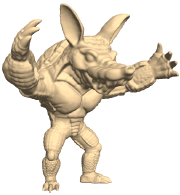
\includegraphics[clip,scale=0.4]{imagens/Olga_Sorkine_3.png} 
\end{center}
\end{figure} 
\end{frame} 
 
%%%%%%%%%%%%%%%%%%%%%%%%%%%%%%%%%%%%%%%%%%%%%%%%%%%%%%%%%%%%%%%%%%%%%%%%%%%%%%%%%%%

\pgfdeclareimage[height=1.8cm]{logo}{imagens/olga.png} 
\logo{\pgfuseimage{logo}}

%%%%%%%%%%%%%%%%%%%%%%%%%%%%% SUMARIO %%%%%%%%%%%%%%%%%%%%%%%%%%%%%%%%%%%%%%

\begin{frame}[allowframebreaks]
\frametitle{Sumário}
\tableofcontents
\end{frame}

%%%%%%%%%%%%%%%%%%%%%%%%%%%%%%%%%%%%%%%%%%%%%%%%%%%%%%%%%%%%%%%%%%%%%%%%%%%%%%%%%%%
\centering

%%%%%%%%%%%%%%%%%%%%%%%%%%%%%%%%%%%%%%%%%%%%%%%%%%%%%%%%%%%%%%%%%%%%%%%%%%%%%%%%%%%
%%%%%%%%%%%%%%%%%%%%%%%%%%%%%%%%%%%%%%%%%%%%%%%%%%%%%%%%%%%%%%%%%%%%%%%%%%%%%%%%%%%
\section{Modelagem geométrica}
\begin{frame}
\frametitle{Resumo do projeto}
\framesubtitle{Introdução}

\begin{figure}[hbt]
	\begin{center}
		\caption{Diagrama de bloco das etapas de desenvolvimento}
		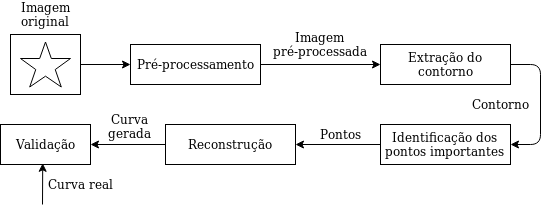
\includegraphics[width=1\textwidth]{img/diagrama.png}
	\end{center}
\end{figure}

\end{frame}


\begin{frame}
	\frametitle{Resumo do projeto}
	\framesubtitle{Exemplo (simples)}
	
	\begin{figure}[ht!]
		\centering
		\begin{subfigure}[b]{0.19\textwidth}
			\centering
			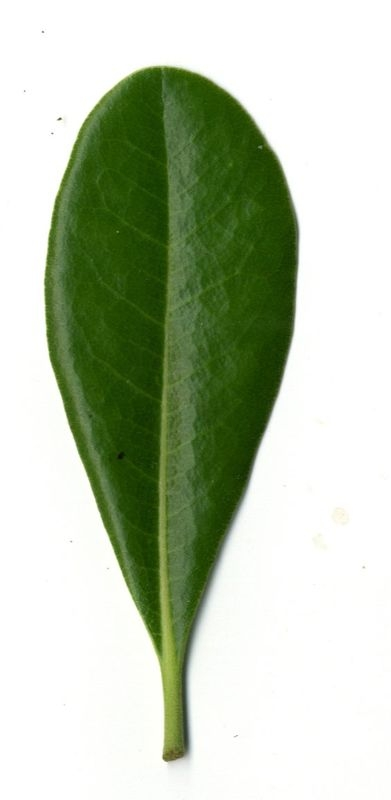
\includegraphics[width=\textwidth]{img/original.jpg}
		\end{subfigure}
		\begin{subfigure}[b]{0.19\textwidth}
			\centering
			
\includegraphics[width=\textwidth]{img/preprocess.jpg}
		\end{subfigure}
		\begin{subfigure}[b]{0.19\textwidth}
			\centering
			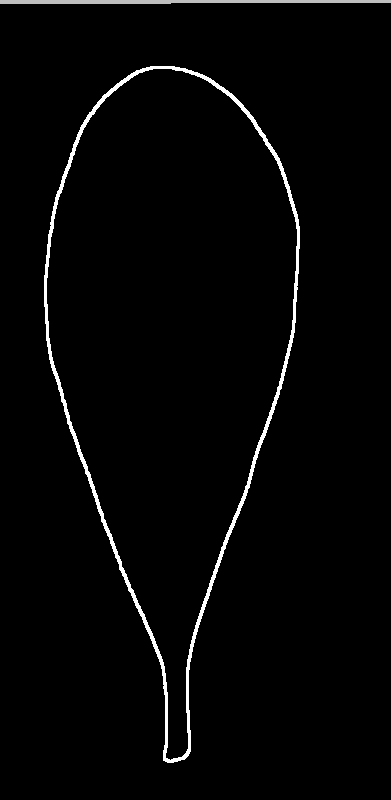
\includegraphics[width=\textwidth]{img/contour.jpg}
		\end{subfigure}
		\begin{subfigure}[b]{0.19\textwidth}
			\centering
			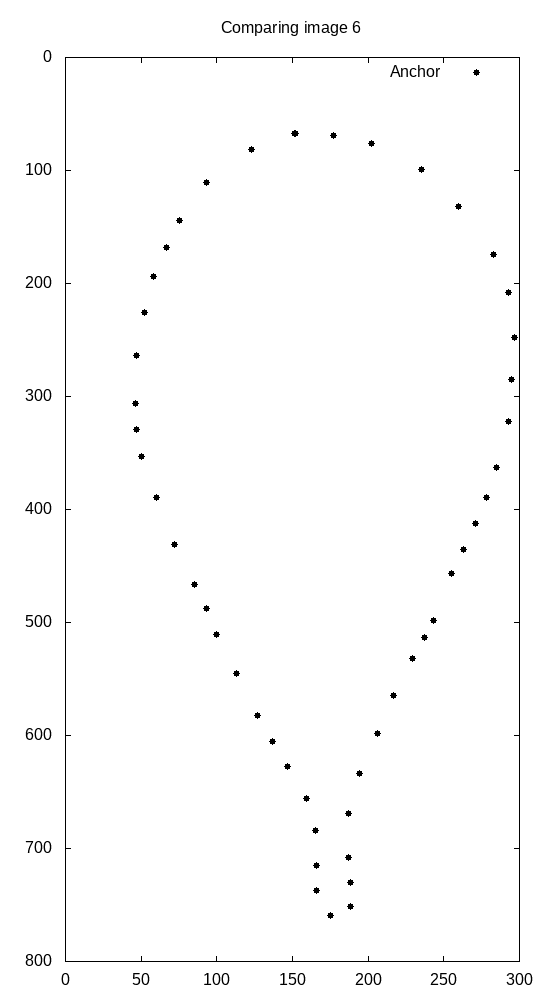
\includegraphics[width=\textwidth]{img/points.png}
		\end{subfigure}
		\begin{subfigure}[b]{0.19\textwidth}
			\centering
			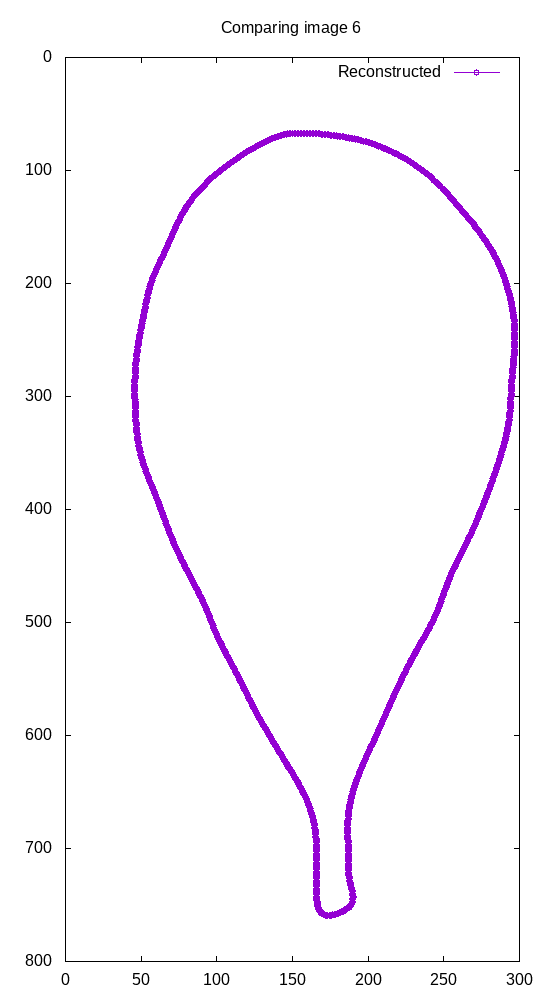
\includegraphics[width=\textwidth]{img/reconstructed.png}
		\end{subfigure}
		\label{fig:editedmesh}
	\end{figure}
	
\end{frame}




\section{Definições}
\begin{defi}[Operador de Laplace]
Seja $f$ uma função duplamente derivável de valores reais no espaço euclidiano $\mathbb{R}^n$. O \textbf{operador de Laplace} (também conhecido como Laplaciano), denotado por $\Delta$ ou $\nabla^2$, é definido como o divergente do gradiente:
\begin{equation}
\Delta f = \nabla^2 f = \nabla \cdot (\nabla f) = \text{div} (\text{grad f})
\end{equation}
\end{defi}

A denominação de \textbf{operador de Laplace-Beltrami} vem no contexto de geometria diferencial, em que o Laplaciano pode ser generalizado para operar sobre funções definidas em subvariedades no espaço euclideano e, mais genericamente, em variedades Riemannianas e pseudo-Riemannianas.

\begin{defi}[Coordenadas diferenciais]
	Seja uma malha triangular de $n$ vértices caracterizada por $\mathcal{M} = (V, E, F)$, em que $V, A, F$ são, respectivamente, os conjuntos de seus vértices, arestas e faces. Cada vértice $\mathbf{v}_i \in V$ possui uma representação cartesiana dada por $\mathbf{v}_i = (x_i,y_i,z_i)$. \textbf{Coordenadas diferenciais} (também conhecidas como $\mathbf{\delta}$\textit{-coordenadas}) de $\mathbf{v}_i$ são definidas como a diferença entre a coordenada cartesiana e o centro de massa de seus vizinhos imediatos na malha:
	
	\begin{equation}
	\mathbf{\delta}_i = (\mathbf{\delta}_i^{(x)}, \mathbf{\delta}_i^{(y)}, \mathbf{\delta}_i^{(z)}) = \mathbf{v}_i - \frac{1}{d_i} \sum_{j \in N(i)} \mathbf{v}_j,
	\label{eq_delta}
	\end{equation}
	
	\noindent em que $N(i) = \{j|(i,j) \in E$\} (ou seja, os vértices adjacentes a $i$) e $d_i = |N(i)|$ é o número dos vizinhos imediatos de $i$ (grau de $i$).
\end{defi}

A transformação do vetor de coordenadas cartesianas absolutas ao vetor das $\mathbf{\delta}$-coordenadas, descrita na equação \ref{eq_delta}, também pode ser representada em forma de matriz. Seja $A$ a matriz de adjacências da malha:

\begin{equation}\label{eqMatAdj}
A_{ij} = \begin{cases}
1&(i, j) \in E\\
0&\text{caso contrário.}
\end{cases}
\end{equation}

\noindent e $D$ matriz diagonal tal que $D_{ii} = d_i$ (grau de incidência do nó $i$). Assim, a matriz transformação de coordenadas absolutas para as coordenadas relativas é:

\begin{equation}
L = I - D^{-1}A.
\end{equation}

É mais conveniente utilizar a versão simétrica $L_s$ da matriz $L$, definida por:

\begin{equation}\label{eqMatLaplaciana}
L_s = DL = D - A
\end{equation}

\noindent em que cada célula pode ser calculada da seguinte forma:

\begin{equation}
(L_s)_{ij} = \begin{cases}
d_i&i=j\\
-1&(i, j) \in E\\
0&\text{caso contrário.}
\end{cases}
\end{equation}

A matriz $L_s$ é denominada \textit{Laplaciano topológico} da malha $\mathcal M$. A figura \ref{fig:matrizLaplaciana} ilustra um exemplo de uma simples malha triangular e sua respectiva representação matricial Laplaciana.

\begin{figure}[htb]
	\centering
	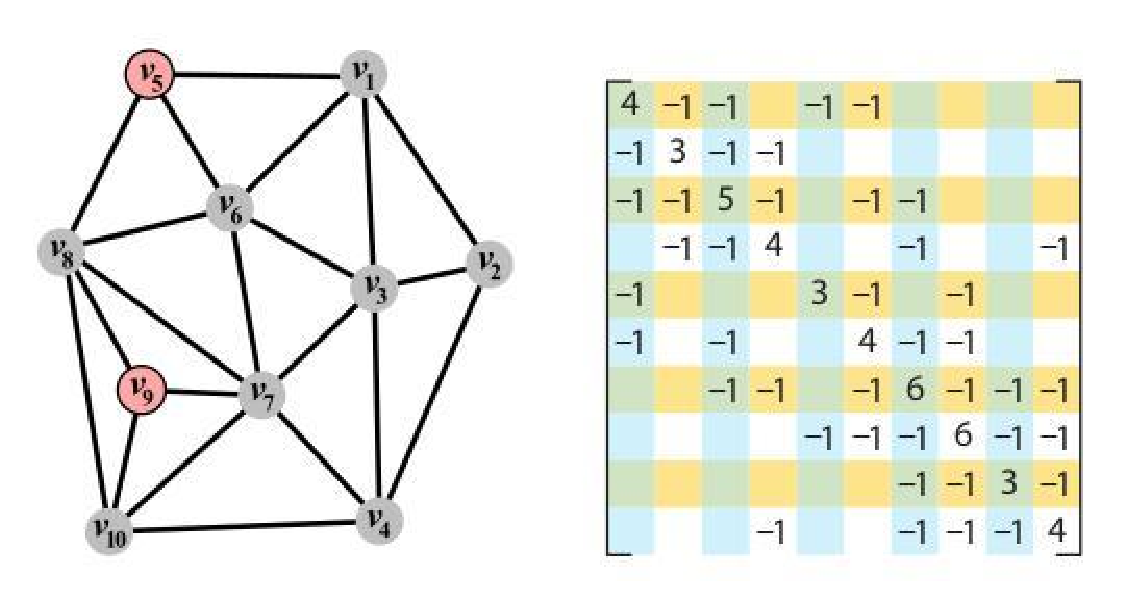
\includegraphics[width=.5\linewidth]{imagens/cap4/meshLaplacian.eps}
	\caption{Uma malha triangular e sua respectiva matriz Laplaciana $L_s$ \cite{sorkine2006}}
	\label{fig:matrizLaplaciana}
\end{figure}

Caso a malha $\mathcal{M}$ seja a aproximação linear por partes de uma superfície suave, as $\mathbf{\delta}$-coordenadas podem ser vistas como a discretização do operador contínuo de Laplace-Beltrami. Pode-se denotar o vetor de coordenadas diferenciais em um vértice $v_i$ como

\begin{equation}
\mathbf{\delta}_i = \frac{1}{d_i} \sum_{j \in N(i)} (\mathbf{v}_i - \mathbf{v}_j)
\end{equation}

\noindent em que este somatório é a discretização da seguinte integral:

\begin{equation}
\frac{1}{|\gamma|} \int_{\mathbf{v} \in \gamma} (\mathbf{v}_i - v) dl(\mathbf{v}))
\end{equation}

\noindent onde $\gamma$ é uma superfície simples e fechada em torno de $\mathbf{v}$ e $|\gamma|$ é o comprimento de $\gamma$. Sabe-se que

\begin{equation}
	\lim_{|\gamma| \rightarrow 0} \frac{1}{|\gamma|} \int_{\mathbf{v} \in \gamma} (\mathbf{v}_i - \mathbf{v}) dl(\mathbf{v}) =  -H(\mathbf{v}_i)\mathbf{n}_i
\end{equation}


\noindent em que $H(\mathbf{v}_i)$ é a curvatura média em $\mathbf{v}_i$ e $\mathbf{n}_i$ é o vetor normal à superfície. Assim, a direção do vetor de coordenadas diferenciais aproxima a direção normal e sua norma aproxima a quantidade proporcional à curvatura média local (o vetor normal escalado pela curvatura média é dito normal da curvatura média). Intuitivamente, isto significa que as $\mathbf{\delta}$-coordenadas encapsulam a forma da superfície local.

Portanto, como ilustra a figura \ref{fig:coordDif}, as coordenadas diferenciais aproximam não apenas as características da forma local da superfície, mas também a direção normal e a curvatura média. 

\begin{figure}[htb]
	\centering
	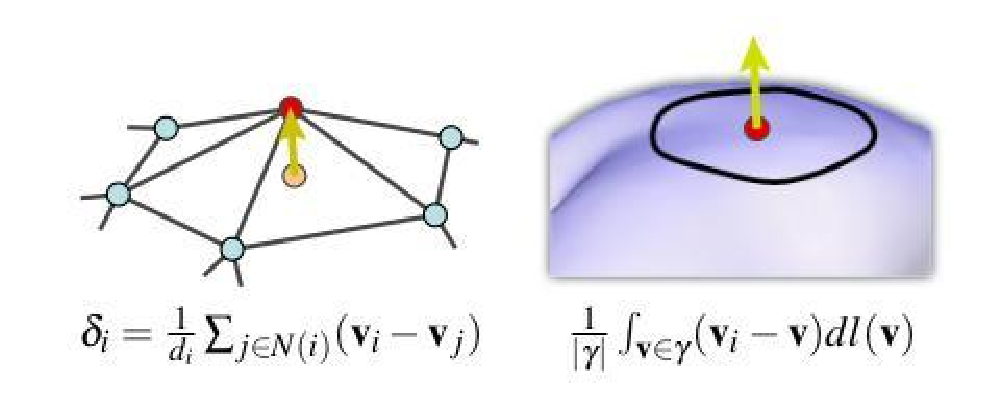
\includegraphics[width=.7\linewidth]{imagens/cap4/difcoord.eps}
	\caption{O vetor da coordenada diferencial em um vértice aproxima a forma local superfície: representação da direção normal e da curvatura média \cite{sorkine2006}}
	\label{fig:coordDif}
\end{figure}

Existem outras formas de se calcular as $\delta$-coordenadas, de forma a se obter melhores qualidades de aproximação. Por exemplo, pode-se ponderar geometricamente o somatório com cotangentes \cite{pinkall:1996}:

\begin{equation}
	\mathbf{\delta}_i^c = \frac{1}{|\Omega|} \sum_{j \in N(i)} \frac{1}{2} (\cot \alpha_{ij} + \cot \beta_{ij})(\mathbf{v}_i - \mathbf{v}_j))
\end{equation}

\noindent em que $|\Omega|$ é o tamanho da célula de Voronoi de $i$ e $\alpha_{ij}, \beta_{ij}$ são os dois ângulos opostos à aresta $(i, j)$. Esta ponderação gera os vetores $\mathbf{\delta}_i^c$, que possuem apenas componentes normais (ao contrário das $\mathbf{\delta}$-coordenadas definidas anteriormente, que podem possuir componentes tangenciais e serem não nulas em 1-anéis planares). Porém, os valores das cotangentes podem ser negativos ou possuírem alguns problemas (em ângulos com valores se aproximando de $\pi$).


\section{Aplicações}
%%%%%%%%%%%%%%%%%%%%%%%%%%%%%%%%%%%%%%%%%%%%%%%%%%%%%%%%%%%%%%%%%%%%%%%%%%%%%%%%%%%
\subsection{Representação eficiente de formas}
%%%%%%%%%%%%%%%%%%%%%%%%%%%%%%%%%%%%%%%%%%%%%%%%%%%%%%%%%%%%%%%%%%%%%%%%%%%%%%%%%%%

%%%%%%%%%%%%%%%%%%%%%%%%%%%%% SLIDE 4.0 %%%%%%%%%%%%%%%%%%%%%%%%%%%%%%%%%%%%%%%%%%%
\begin{frame}
\frametitle{{\bf \color{blue} Aplicações}}
	
\begin{block}{\bf Representação eficiente de formas}
Se utilizada uma boa base para representação, é necessária apenas uma parcela da função de base para representar toda a geometria.
\end{block}

\begin{center}
	\begin{figure}
	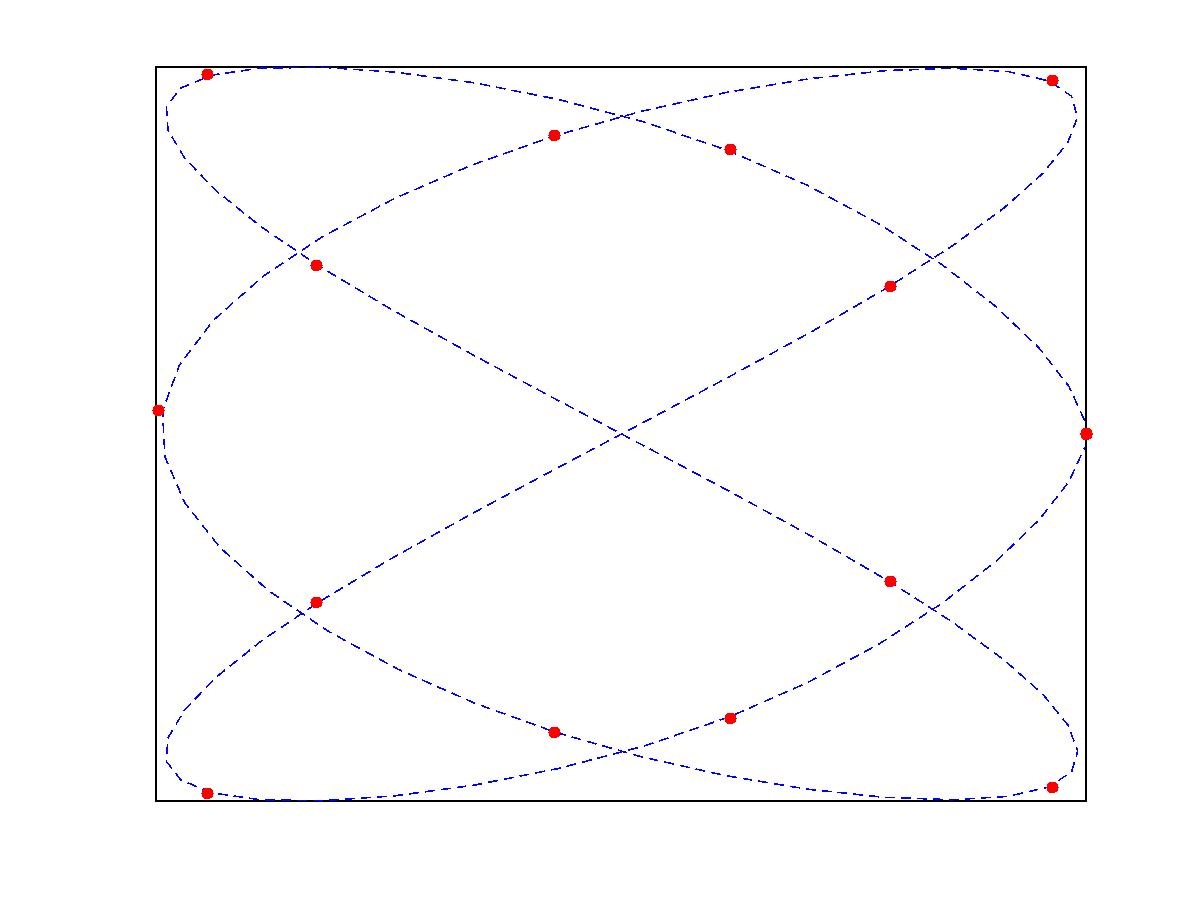
\includegraphics[trim={4cm, 3cm, 4cm, 2cm},clip,width=0.4\linewidth]{imagens/rep_dashed.jpg}
	\caption{Função paramétrica estimada a partir dos pontos em vermelho (âncora) e de informações de conectividade da malha.}
	\end{figure}
\end{center}
	
\end{frame}

\begin{frame}
\frametitle{{\bf \color{blue} Aplicações}}
\framesubtitle{\color{blue} Representação eficiente de formas}
	
	\begin{block}{\bf Representação eficiente de formas}
		Com apenas informações de conectividade da malha e alguns pontos fixados (denominados vértices âncora), é possível aproximar toda a geometria, a partir da resolução do sistema pelo método dos mínimos quadrados:
		
		\begin{equation}\label{eq:sisrecover}
			\left( \frac{L}{\omega I_{m \times m} | 0} \right) \mathbf{x'} = \begin{pmatrix}
				0\\
				\omega\ c_{1:m}^{(x)}
			\end{pmatrix}
		\end{equation}
		
		em que $c = \{v_1, v_2, \dots, v_m\}$ são os pontos âncora escolhidos como amostra, e $\omega > 0$ é o peso de cada restrição).
	\end{block}
	
\end{frame}

\begin{frame}
	\frametitle{{\bf \color{blue} Aplicações}}
	\framesubtitle{\color{blue} Representação eficiente de formas}
	
	\begin{block}{\bf Representação eficiente de formas}
		Graficamente, para facilitar a visualização, este sistema matricial também pode ser visto deste jeito:
		
		\begin{center}
			\begin{tikzpicture}
				\filldraw[fill=olive!40!white, draw=black] (0,-0.8) rectangle node{$\tilde{L}$} (2,2);
				\filldraw[fill=blue!30!white, draw=black] (2.1,0) rectangle node{$x$} (3.1,2);
				\draw (3.4, 0.95) -- (3.7, 0.95);
				\draw (3.4, 1.05) -- (3.7, 1.05);
				\filldraw[fill=purple!30!white, draw=black] (4,0) rectangle node{$0$} (6,2);
				\filldraw[fill=purple!50!white, draw=black] (4,0) rectangle node{$v_c$} (6,-0.8);
			\end{tikzpicture}
		\end{center}
		
	\end{block}
	
\end{frame}


\begin{frame}
\frametitle{{\bf \color{blue} Aplicações}}
\framesubtitle{\color{blue} Representação eficiente de formas}
	
\begin{block}{\bf Reconstrução - observações}
Em vez de $\delta^{(x)}$ do lado direito, informa-se $0$ nas coordenadas em que não sabe a localização.

\medskip

Estas localizações serão calculadas por informações das malhas, descritas na matriz $\tilde{L}$.

\medskip

Por isso, é importante que se tenha conhecimento de informações de conectividade da malha em análise.
\end{block}
\end{frame}


\begin{frame}[fragile]
\frametitle{{\bf \color{blue} Aplicações}}
\framesubtitle{\color{blue} Representação eficiente de formas}

\begin{block}{\bf Reconstrução - observações}
Caso se saiba que a malha é, por exemplo, uma curva contínua e fechada no $\mathbb{R}^2$, pode-se utilizar o seguinte código para geração da matriz de adjacências:
\end{block}

\begin{Codigo}[geração de matriz de adjacências]
\noindent\rule{11.2cm}{1.pt}
\vspace{-0.2cm}
\begin{verbatim}
function [ A ] = geraAdjacenciaPadrao(n)
 % Entrada:
 %   n: numero de vertices
 A = zeros(n);
 for i=1:n
   A(i,mod(i-2, n)+1) = 1;
   A(i,mod(i, n)+1) = 1;
 end
end
\end{verbatim}\\
\vspace{-0.5cm}
\noindent\rule{11.2cm}{1.pt}\\
\end{Codigo}
\end{frame}


\begin{frame}[fragile]
\frametitle{{\bf \color{blue} Aplicações}}
\framesubtitle{\color{blue} Representação eficiente de formas}

\begin{Codigo}[reconstrução de curva a partir de poucos pontos]
\noindent\rule{11.2cm}{1.pt}
\vspace{-0.2cm}
\begin{verbatim}
n = 100; % numero de pontos no total
n_coords = 2; % dimensao
t = linspace(0, 2*pi, n); % dominio
v = [cos(t) + sin(t); cos(t)]; % v(x, y)'; % v(x, y)

n_known = 11; % reconstrucao com pontos linearmente espacados
known = round(linspace(1, n, n_known));
v_known = zeros(n, n_coords);
v_known(known,:) = v(known,:);

A = geraAdjacenciaPadrao(n);
Ls = geraLaplaciano(A);
delta = zeros(n, n_coords);
recovered = recuperaCoords(Ls, delta, known, v_known(known,:))
\end{verbatim}\\
\vspace{-0.5cm}
\noindent\rule{11.2cm}{1.pt}\\
\end{Codigo}
\end{frame}


\begin{frame}
\frametitle{{\bf \color{blue} Aplicações}}
\framesubtitle{\color{blue} Representação eficiente de formas}

\begin{figure}
	\centering
	\begin{subfigure}[b]{0.31\textwidth}
		\centering
		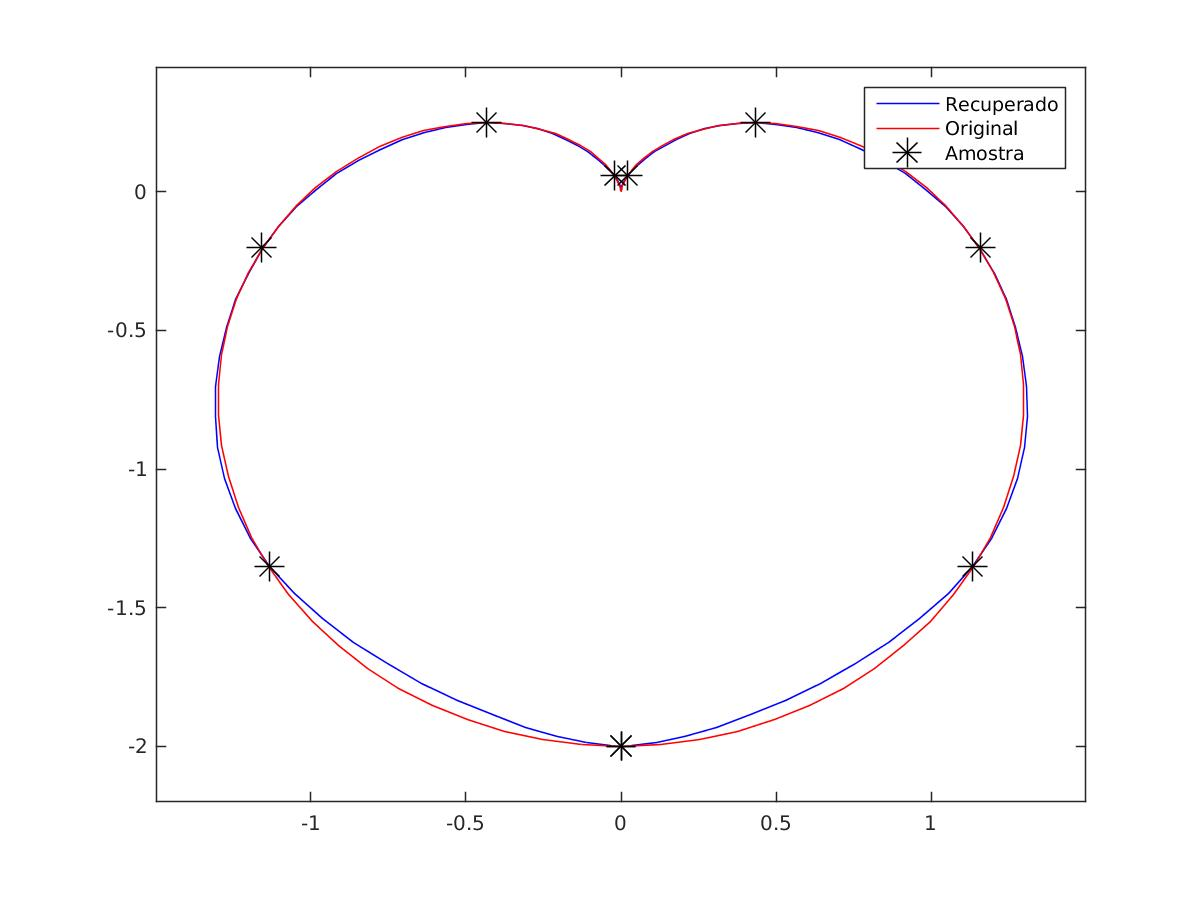
\includegraphics[trim={5cm 2cm 3cm 2cm},clip,width=\textwidth]{imagens/rep_1_10.jpg}
		\caption{10 pontos}
		\label{fig:ex14}
	\end{subfigure}
	\hfill
	\begin{subfigure}[b]{0.31\textwidth}
		\centering
		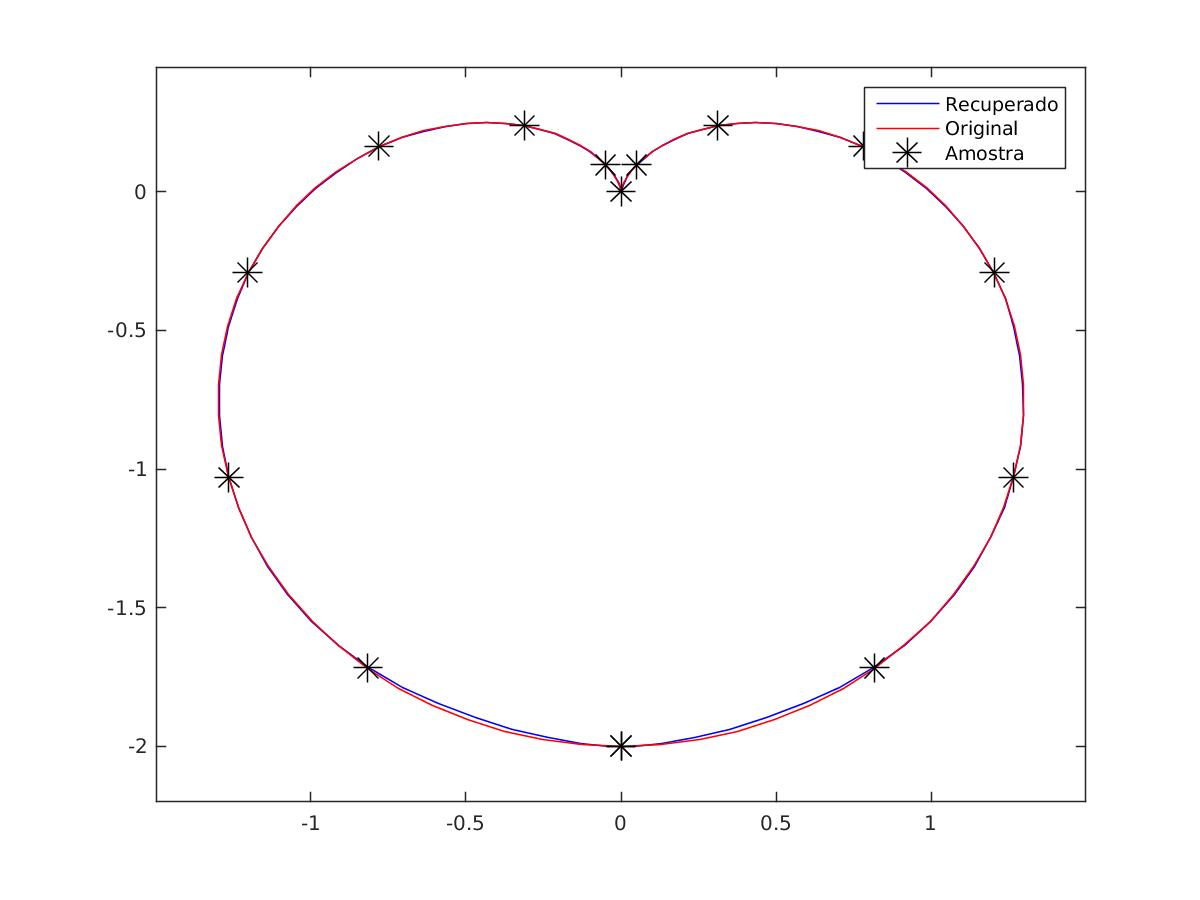
\includegraphics[trim={5cm 2cm 3cm 2cm},clip,width=\textwidth]{imagens/rep_1_15.jpg}
		\caption{15 pontos}
		\label{fig:ex12}
	\end{subfigure}
	\hfill
	\begin{subfigure}[b]{0.31\textwidth}
		\centering
		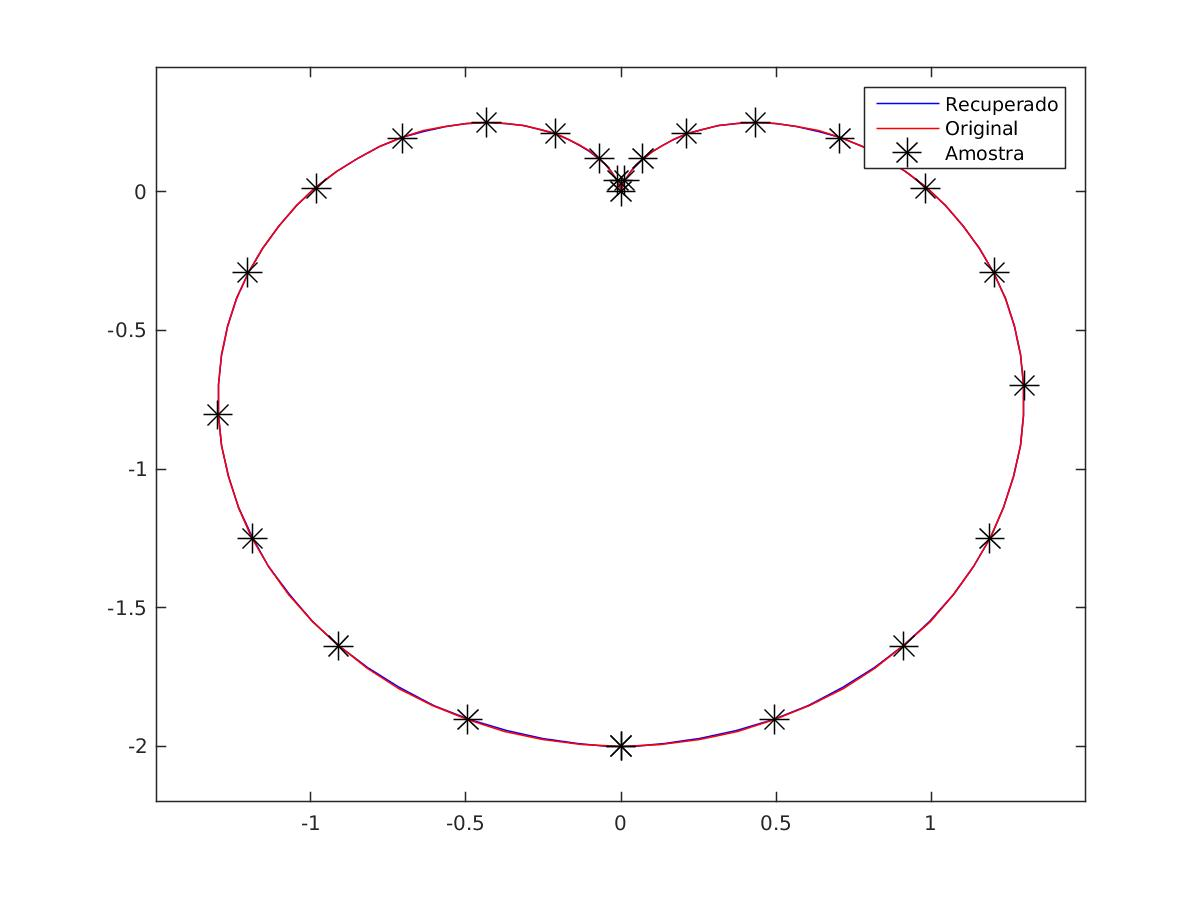
\includegraphics[trim={5cm 2cm 3cm 2cm},clip,width=\textwidth]{imagens/rep_1_25.jpg}
		\caption{25 pontos}
		\label{fig:ex13}
	\end{subfigure}
	\caption{Representação da função paramétrica $(x(t), y(t)) = (sin(t) + 0.5 sen(2t), -cos(t) - 0.5 - 0.5 cos(2t))$ utilizando alguns pontos igualmente espaçados como amostra.}
	\label{fig:ex1rep}
\end{figure}

\end{frame}


\begin{frame}
\frametitle{{\bf \color{blue} Aplicações}}
\framesubtitle{\color{blue} Representação eficiente de formas}

\begin{figure}
	\centering
	\begin{subfigure}[b]{0.31\textwidth}
		\centering
		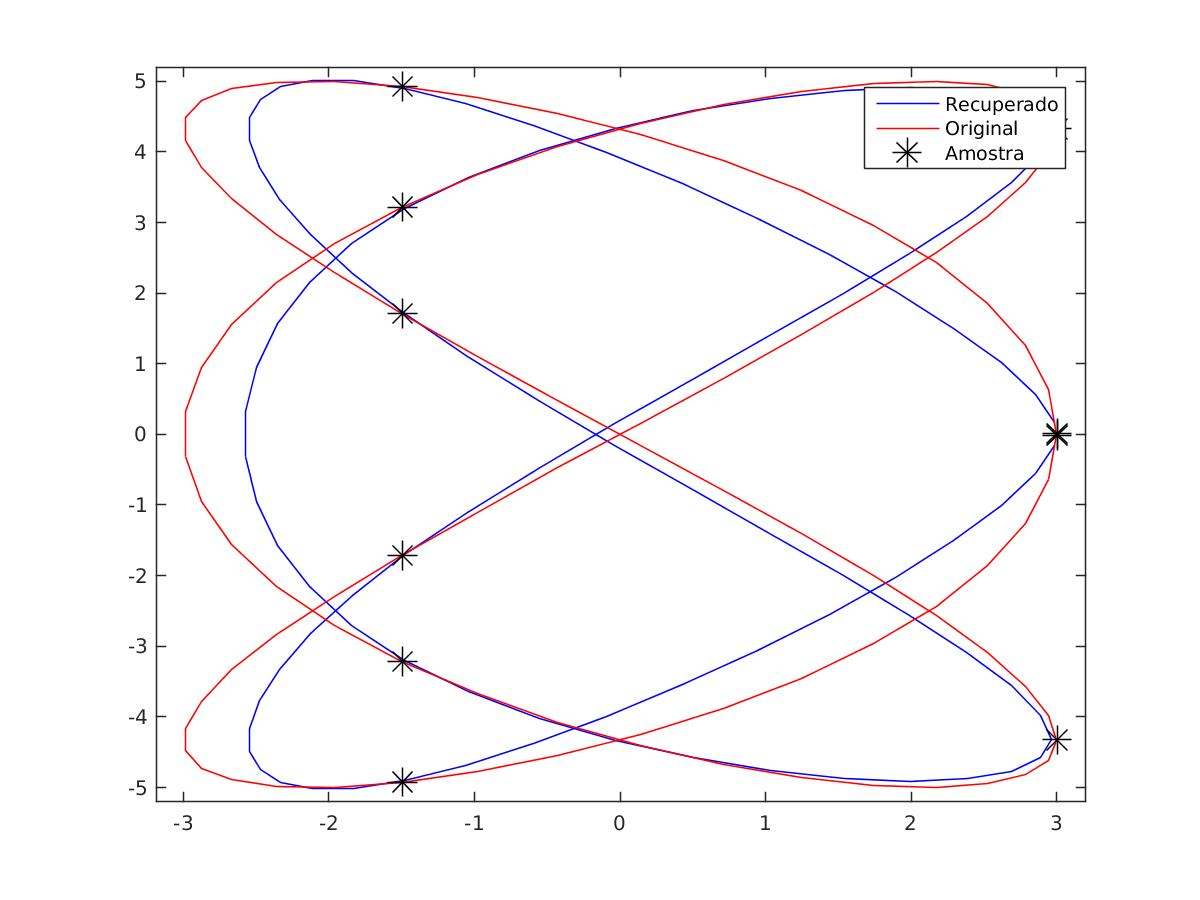
\includegraphics[trim={5cm 2cm 3cm 2cm},clip,width=\textwidth]{imagens/rep_2_10.jpg}
		\caption{10 pontos}
		\label{fig:ex24}
	\end{subfigure}
	\hfill
	\begin{subfigure}[b]{0.31\textwidth}
		\centering
		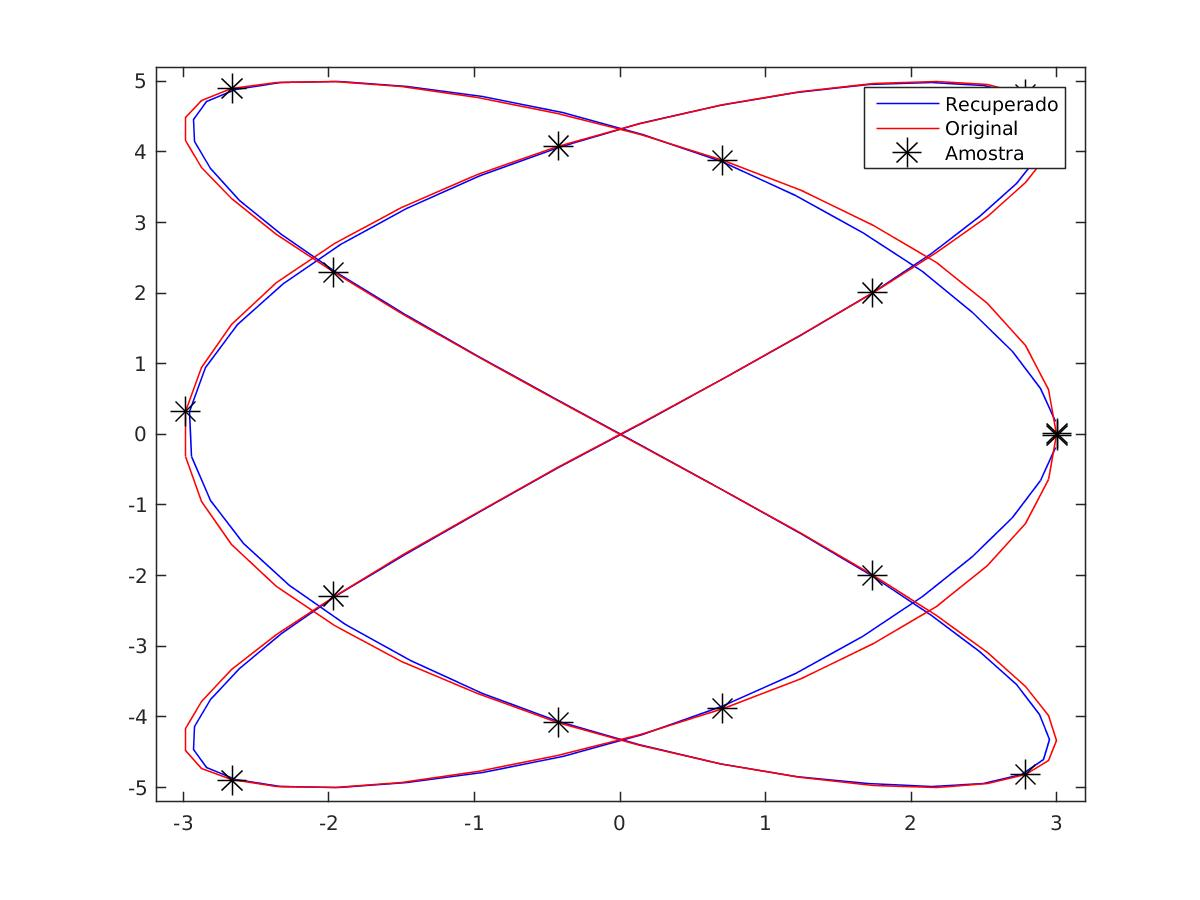
\includegraphics[trim={5cm 2cm 3cm 2cm},clip,width=\textwidth]{imagens/rep_2_15.jpg}
		\caption{15 pontos}
		\label{fig:ex22}
	\end{subfigure}
	\hfill
	\begin{subfigure}[b]{0.31\textwidth}
		\centering
		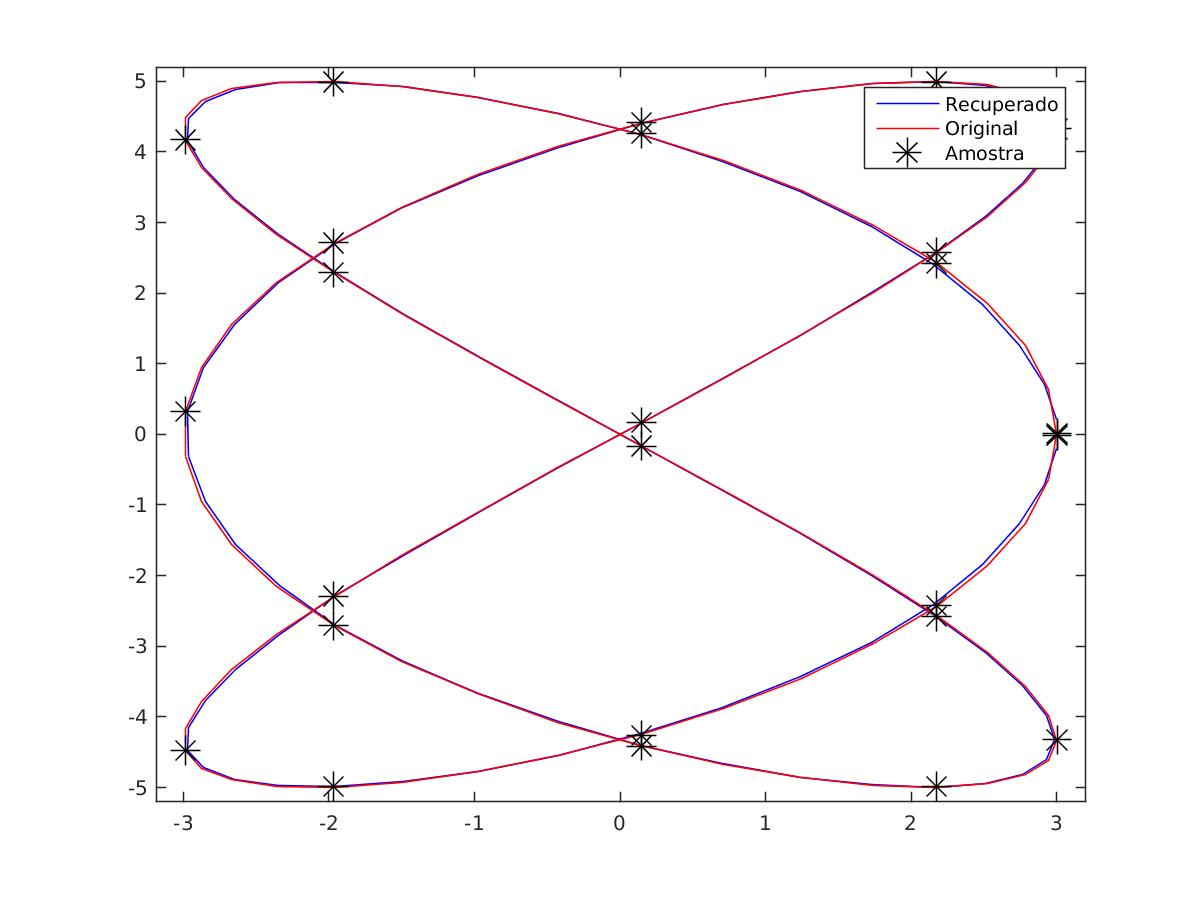
\includegraphics[trim={5cm 2cm 3cm 2cm},clip,width=\textwidth]{imagens/rep_2_25.jpg}
		\caption{25 pontos}
		\label{fig:ex23}
	\end{subfigure} %[3 * cos(3 * t); 5 * sin(2 * t)]';
	\caption{Representação da função paramétrica $(x(t), y(t)) = (3 cos(3t), 5sen(2t))$ utilizando alguns pontos igualmente espaçados como amostra.}
	\label{fig:ex2rep}
\end{figure}


\end{frame}


\begin{frame}
\frametitle{{\bf \color{blue} Aplicações}}
\framesubtitle{\color{blue} Representação eficiente de formas}
	\begin{block}{\bf Reconstrução de superfícies}
		Também é possível representar superfícies lineares por partes a partir de poucas amostras na variedade original.
	\end{block}
	\begin{figure}
		\centering
		\begin{subfigure}[b]{0.49\textwidth}
			\centering
			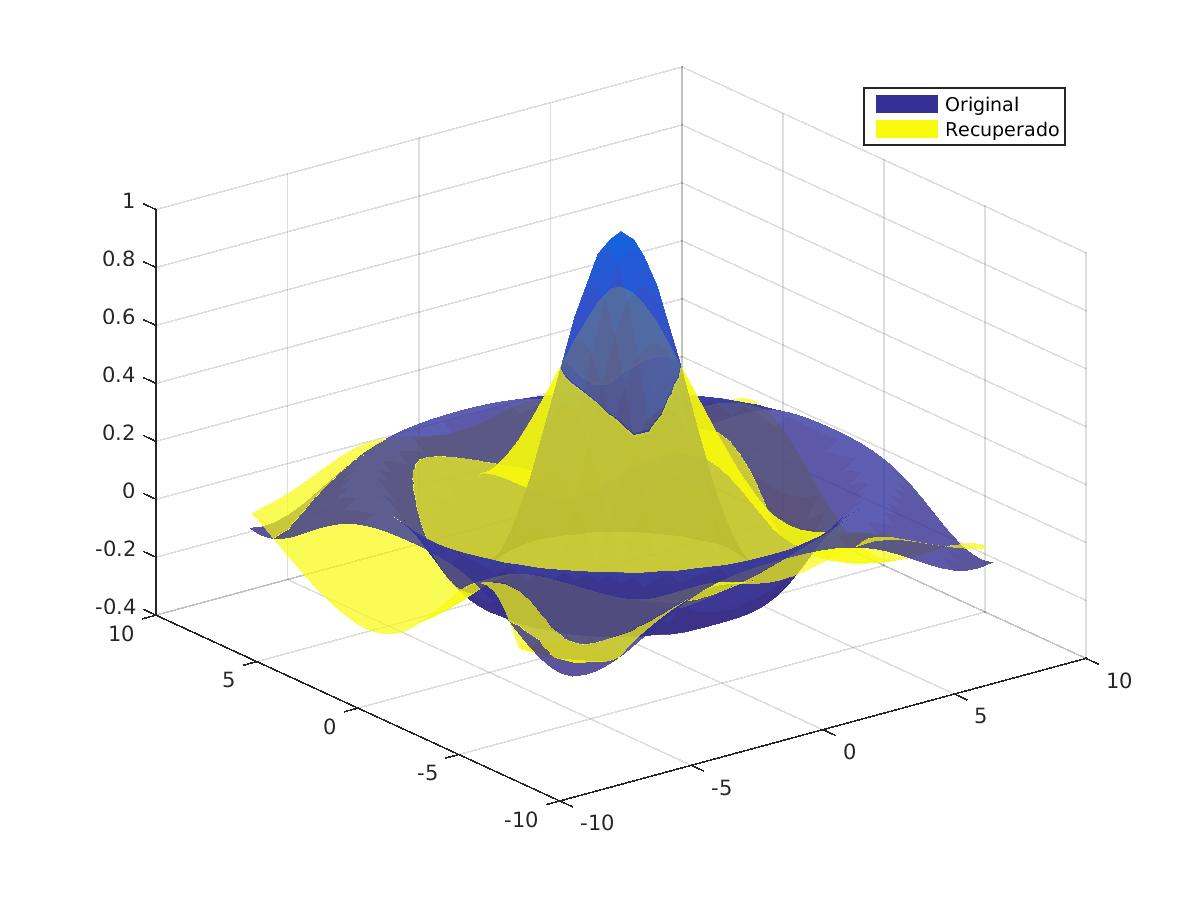
\includegraphics[width=0.9\textwidth]{imagens/rep3_50.jpg}
			\caption{50 pontos}
			\label{fig:surf100}
		\end{subfigure}
		\hfill
		\begin{subfigure}[b]{0.49\textwidth}
			\centering
			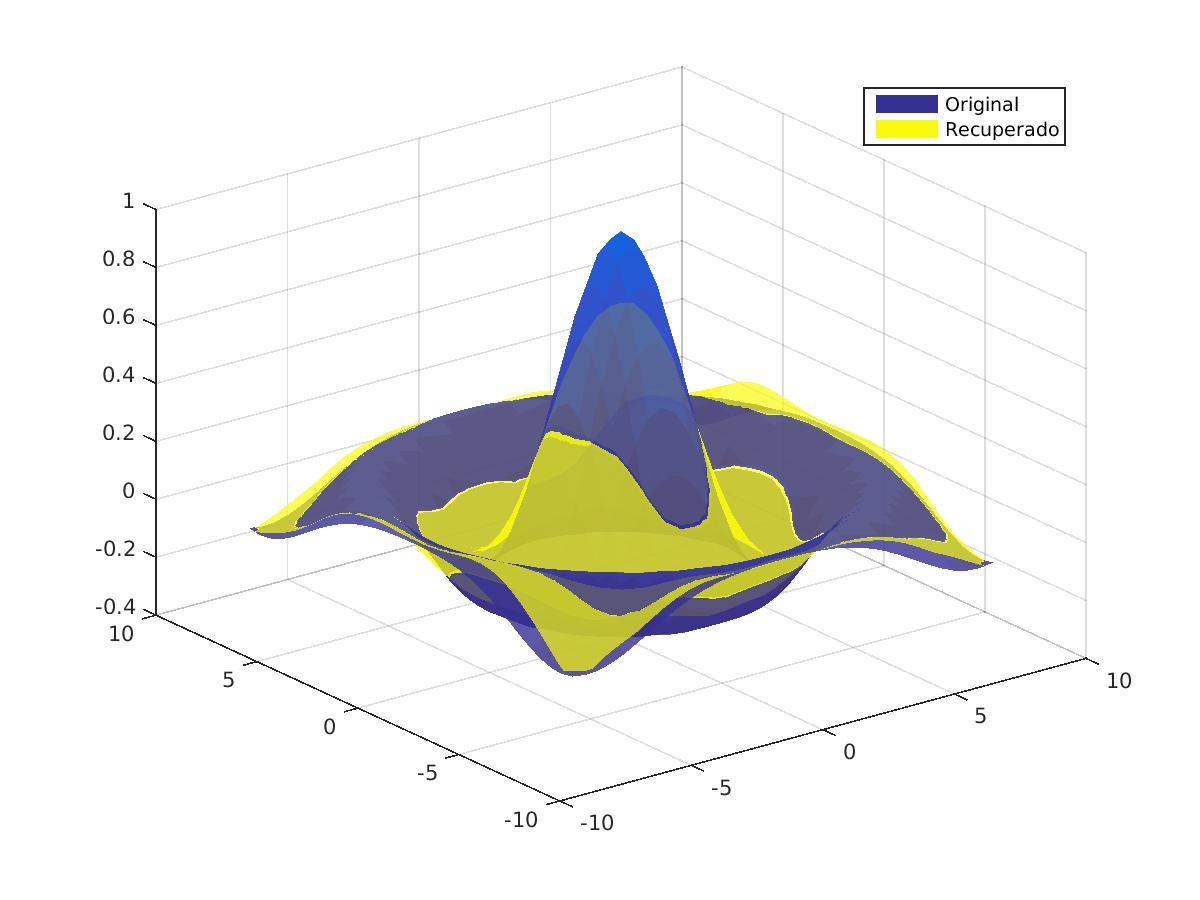
\includegraphics[width=0.9\textwidth]{imagens/rep3_200.jpg}
			\caption{200 pontos}
			\label{fig:surf300}
		\end{subfigure}
		\caption{Reconstrução de superfície utilizando alguns poucos pontos.}
	\end{figure}
	
\end{frame}

%%%%%%%%%%%%%%%%%%%%%%%%%%%%%%%%%%%%%%%%%%%%%%%%%%%%%%%%%%%%%%%%%%%%%%%%%%%%%%%%%%%
\subsection{Edição de malhas e interpolação}
%%%%%%%%%%%%%%%%%%%%%%%%%%%%%%%%%%%%%%%%%%%%%%%%%%%%%%%%%%%%%%%%%%%%%%%%%%%%%%%%%%%

%%%%%%%%%%%%%%%%%%%%%%%%%%%%% SLIDE 4.0 %%%%%%%%%%%%%%%%%%%%%%%%%%%%%%%%%%%%%%%%%%%
\begin{frame}
\frametitle{{\bf \color{blue} Aplicações}}
	
\begin{block}{\bf Edição de malhas}
	Outra interessante aplicação é a de edições de malhas, como movimentos e deformações.
\end{block}

\begin{center}
	\begin{figure}
		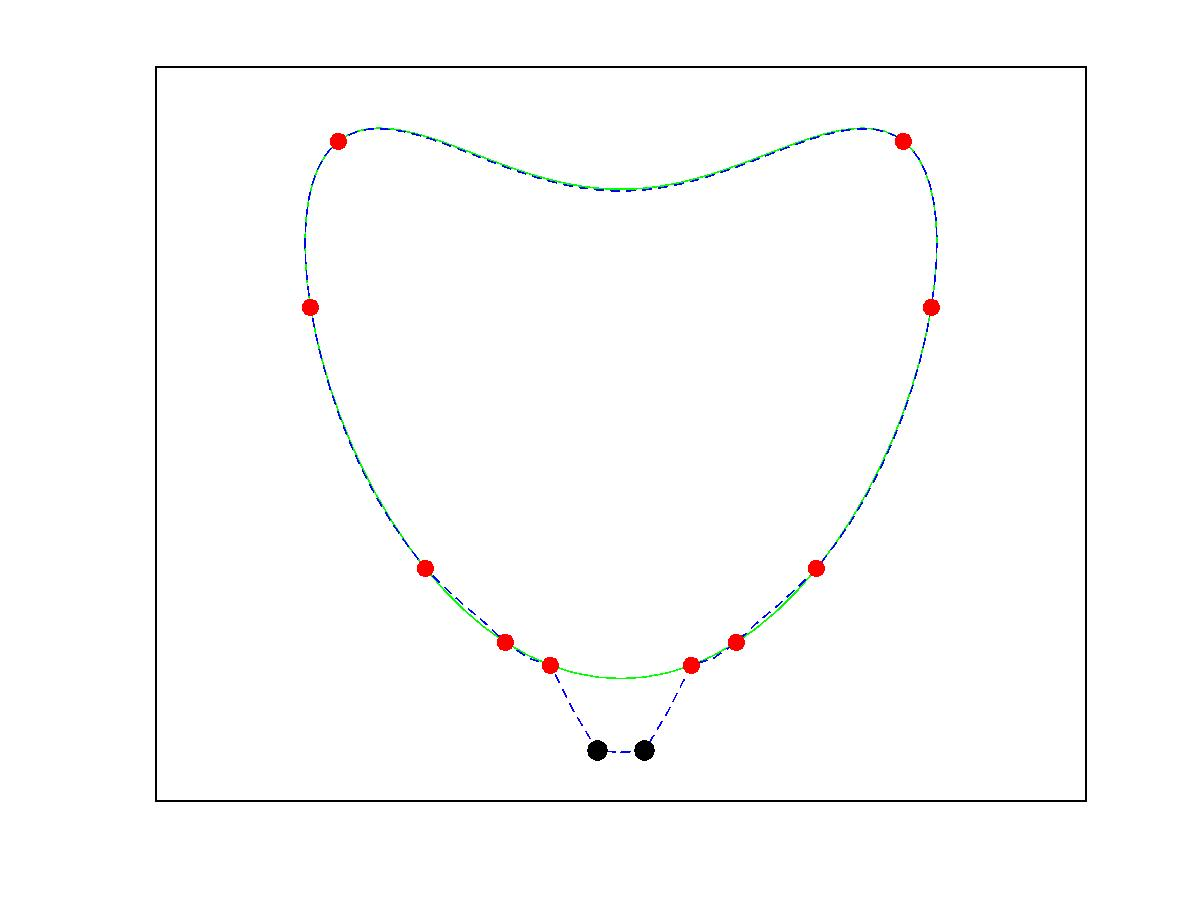
\includegraphics[trim={4cm, 3cm, 4cm, 2cm},clip,width=0.5\linewidth]{imagens/edi_dashed.jpg}
		\caption{Malha original (verde), malha editada (vermelho), pontos âncora (vermelho) e pontos de edição (preto)}
	\end{figure}
\end{center}

\end{frame}

\begin{frame}
	\frametitle{{\bf \color{blue} Aplicações}}
	\framesubtitle{\color{blue} Edição de malhas}
	
	\begin{block}{\bf Edição de malhas}
		Além dos pontos âncoras fixados vistos anteriormente, também são escolhidos alguns pontos de edição, em que se deseja alterar a posição cartesiana, e são adicionadas restrições do tipo:
		
		\begin{align}
			\mathbf{v}_i &= \mathbf{c}_i, &i \in \{1, \dots, m\}\\
			\mathbf{v}_j &= \mathbf{e}_j, &j \in \{m+1, \dots, m+a\}
		\end{align}
		
		\noindent e, matricialmente, o sistema pode ser escrito como:
		
		\begin{equation}\label{eq:sisrecoveredi}
			\left( \frac{L}{\omega I_{(m+a) \times (m+a)} | 0} \right) \mathbf{x'} = \begin{pmatrix}
				\delta^{(x)}\\
				\omega\ c_{1:m}^{(x)}\\
				\omega\ e_{1:a}^{(x)}
			\end{pmatrix}
		\end{equation}
	\end{block}
	
\end{frame}


\begin{frame}
	\frametitle{{\bf \color{blue} Aplicações}}
	\framesubtitle{\color{blue} Edição de malhas}
	
	\begin{block}{\bf Edição de malhas}
		Graficamente, para facilitar a visualização, este sistema matricial também pode ser visto como:
		
		\begin{center}
		\begin{tikzpicture}
			\filldraw[fill=olive!20!white, draw=black] (0,0) rectangle node{$L_s$} (2,2);
			\filldraw[fill=olive!35!white, draw=black] (0,0) rectangle node{$I_c$} (2,-0.8);
			\filldraw[fill=olive!50!white, draw=black] (0,-0.8) rectangle node{$I_e$} (2,-1.6);
			\filldraw[fill=blue!30!white, draw=black] (2.1,0) rectangle node{$\mathbf{x'}$} (3.1,2);
			\draw (3.4, 0.50) -- (3.7, 0.50);
			\draw (3.4, 0.60) -- (3.7, 0.60);
			\filldraw[fill=purple!20!white, draw=black] (4,0) rectangle node{$\delta^{(x)}$} (6,2);
			\filldraw[fill=purple!35!white, draw=black] (4,0) rectangle node{$c^{(x)}$} (6,-0.8);
			\filldraw[fill=purple!50!white, draw=black] (4,-0.8) rectangle node{$e^{(x)}$} (6,-1.6);
		\end{tikzpicture}
		\end{center}
	\end{block}
	
\end{frame}

\begin{frame}
	\frametitle{{\bf \color{blue} Aplicações}}
	\framesubtitle{\color{blue} Edição de malhas}
	
	\begin{block}{\bf Edição - observações}
Como é utilizado o método dos mínimos quadrados para a resolução dos sistemas, talvez aconteça alguns erros de precisão.
		
		\medskip
		
Para minimizar estas falhas, após se encontrar a solução do sistema, pode-se forçar com que $v'_i = v_i$, para alguns $i$, para que pelo menos estes pontos não sofram erros de precisão;
	\end{block}
\end{frame}

\begin{frame}
	\frametitle{{\bf \color{blue} Aplicações}}
	\framesubtitle{\color{blue} Edição de malhas}
	
\begin{figure}[ht!]
	\centering
	\begin{subfigure}[b]{0.47\textwidth}
		\centering
		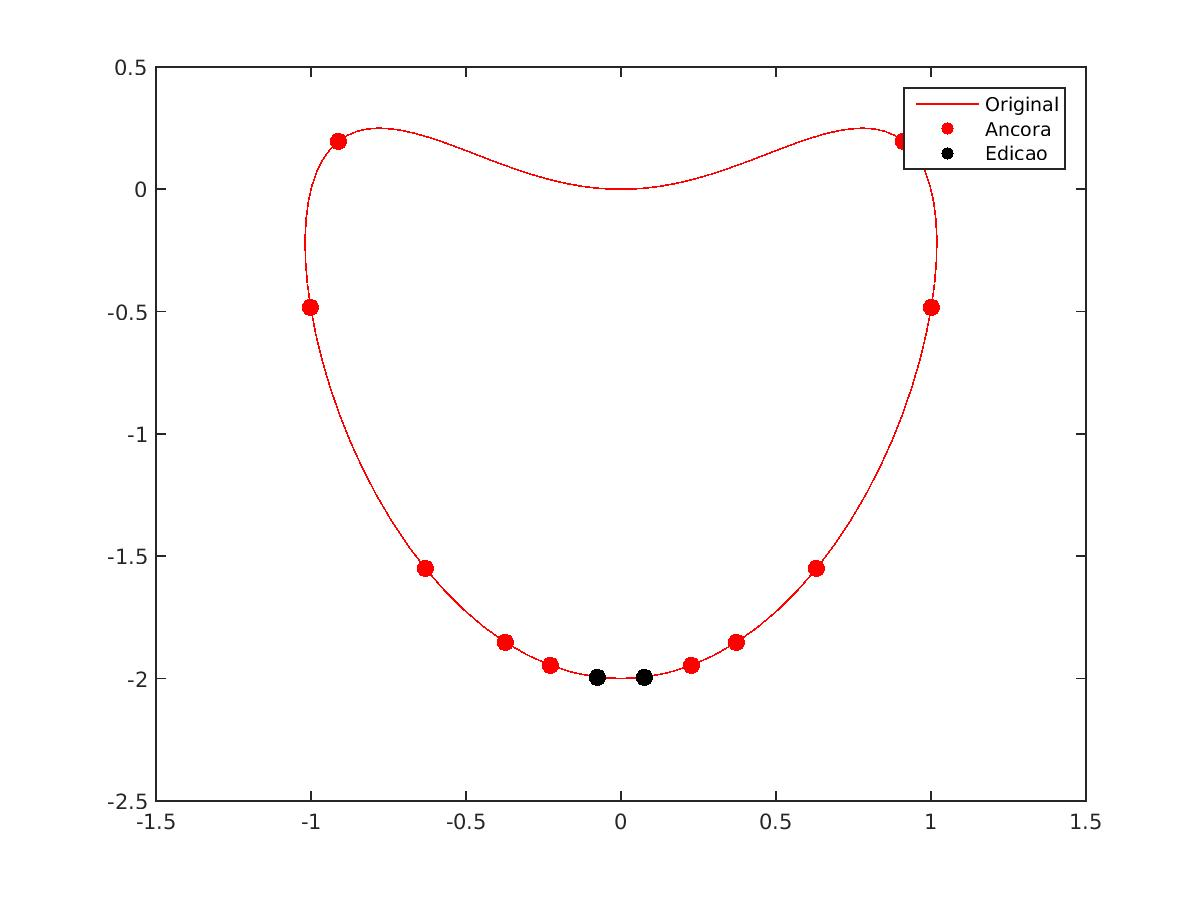
\includegraphics[trim={5cm, 2cm, 3cm, 2cm},clip,width=\textwidth]{imagens/malhaoriginal.jpg}
		\caption{Malha original}
		\label{fig:meshorigiedit}
	\end{subfigure}
	\hfill
	\begin{subfigure}[b]{0.47\textwidth}
		\centering
		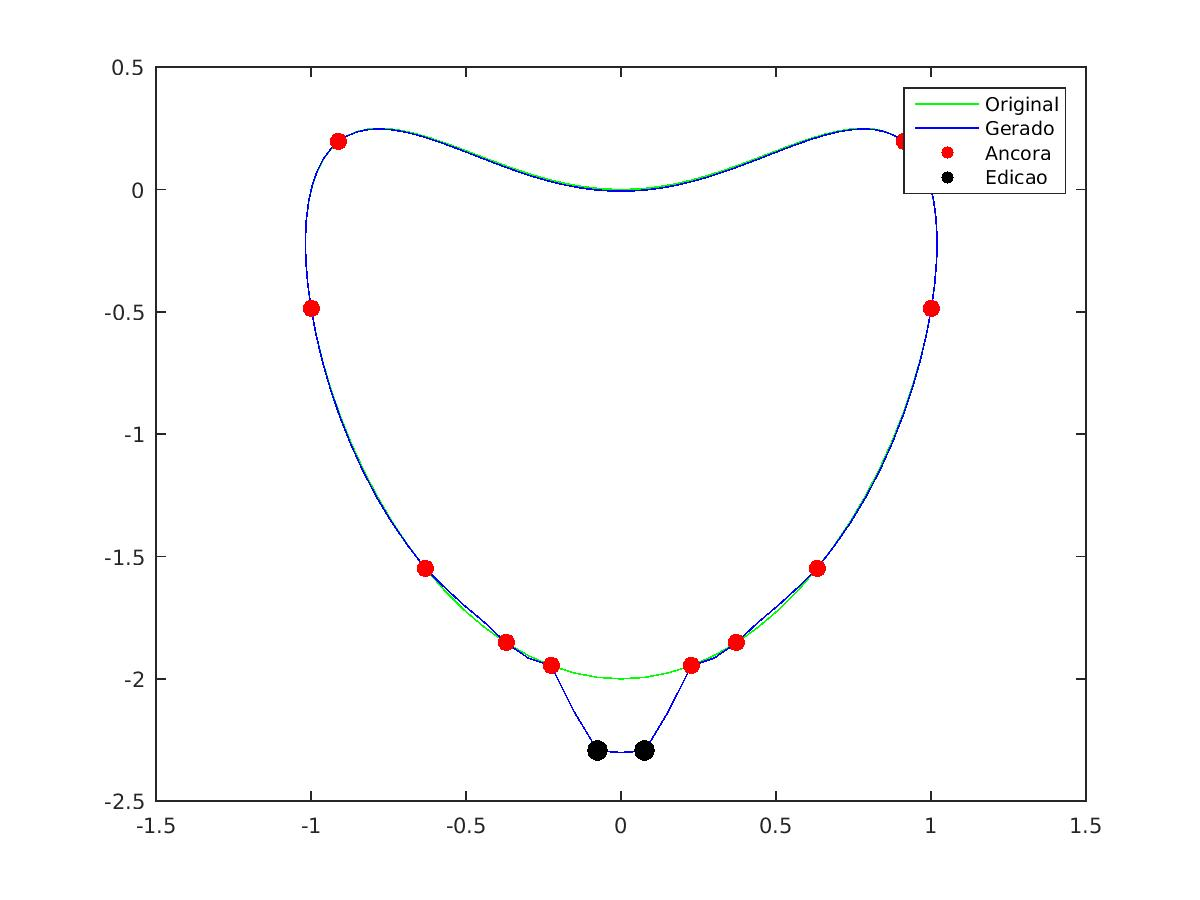
\includegraphics[trim={5cm, 2cm, 3cm, 2cm},clip,width=\textwidth]{imagens/malhaedicao.jpg}
		\caption{Malha editada}
		\label{fig:mesheditededit}
	\end{subfigure}
	\caption{Malha antes e após edição. Os pontos em vermelho são os pontos de âncora, e os pontos em preto são os editados.}
	\label{fig:editedmesh}
\end{figure}

\end{frame}

%%%%%%%%%%%%%%%%%%%%%%%%%%%%%%%%%%%%%%%%%%%%%%%%%%%%%%%%%%%%%%%%%%%%%%%%%%%%%%%%%%%
%%%%%%%%%%%%%%%%%%%%%%%%%%%%%%%%%%%%%%%%%%%%%%%%%%%%%%%%%%%%%%%%%%%%%%%%%%%%%%%%%%%
\section{Referências}

%%%%%%%%%%%%%%%%%%%%%%%%%%%%% Referências %%%%%%%%%%%%%%%%%%%%%%%%%%%%%%%%%%%%%%%%%%%
\begin{frame}[allowframebreaks]{{\bf \color{blue} Referências}}
\nocite{*}
\bibliographystyle{amsalpha}
\bibliography{referencias.bib}
\end{frame}

%%%%%%%%%%%%%%%%%%%%%%%%%%%%%%%%%%%%%%%%%%%%%%%%%%%%%%%%%%%%%%%%%%%%%%%%%%%%%%%%%%%
%%%%%%%%%%%%%%%%%%%%%%%%%%%%%%%%%%%%%%%%%%%%%%%%%%%%%%%%%%%%%%%%%%%%%%%%%%%%%%%%%%%

\end{document} 

 
